%
%
%
\chapter{Computation of the Damped Spin Density Propagator}
\label{appch:propagator}
%
%
%
In the present appendix, the propagator of damped spin density fluctuations is computed, considering the first order in pertubation theory.
Our approach is seperated in two parts.
Firstly, the free spin density propagator is determined, using the equation of motion for Green functions, as suggested in \cite{Elk&Gasser} or many other textbooks.
The damped propagator is then calculated, using the diagrammatic pertubation theory.
The obtained propagator is transformed into Matsubara frquency space, since the computation of the conductivity is treated into there.
%
%
\section{Computation of the Free Propagator}
\label{appsec:free propagator}
%
%
Free propagators are easily computed, using the equation of motion of Green functions.
The equation of motion is obtained, derivating the Green function with respect to the time $t$.
In Fourier space the equation of motion is given by
%
\begin{align}
	\omega \green{\mt{A}}{\mt{B}}_{\omega}^{j} = \expval*{\comm{\mt{A}}{\mt{B}}_{\eta}} + \green{\comm{\mt{A}}{\mt{H}}_{-}}{\mt{B}}_{\omega}^{j},
	\label{appeq: algebraic equation chain}
\end{align}
%
where the typ of the Green function (retarded, advanced and causal) is denoted with $j$ and the frequency dependence of the Green function is represented with an index $\omega$.
The Green function itself is symbolized by double angle brackets.
This equation is an algebraic equation or more precisely an infinite algebraic equation chain for Green functions.
A new more complicated Green function appears on the right hand side.
For this one exists a new equation chain with a more complicted Green function, and so on.
Nevertheless, the equation chain is not infinity in the case of free propagators.

The dynamic of free spin density waves is described by the Hamiltonian $\mt{H}_{\Phi}$ (see equation \eqref{eq:Hamiltonian spin fluctuation}.
The operators A and B are replaced by bosonic field operators $\Phi_{\mu}(\vb{k}+\vb{G},t)$ and $\Phi_{\mu}(-\vb{k}-\vb{G},t)$, respectively.
During the computation, the abbreviation $\green{\Phi_{\mu}}{\Phi_{\mu}}_{\omega}$ is used, where the argument of the field operators is dropped.
The first field operator is always considered with the momentum argument $\vb{k}+\vb{G}$, while the second one has opposite sign.
The time argument is equal for both operators.
The equation of motion is given by
%
\begin{align}
	\omega \green{\Phi_{\mu}}{\Phi_{\mu}}_{\omega} &= 
		\expval{\comm{\Phi_{\mu}(\vb{k}+\vb{G})}{\Phi_{\mu}(-\vb{k}-\vb{G})}}
		+
		\green{\comm{\Phi_{\mu}(\vb{k}+\vb{G})}{\mt{H}_{\Phi}}}{\Phi_{\mu}}_{\omega}
		\label{appeq:equation chain SDW}
\end{align}
%
Both commuators are evaluated on the right hand side, using the bosonic commutator relations.
The inhomogeneity is trivially zero, since the commutator relation is zero per definition.
The commutator, contained in the Green function, is given by
%
\begin{align}
	\comm{\Phi_{\mu}(\vb{k}+\vb{G},t)}{\mt{H}_{\Phi}} &= 
		-\frac{v_{\mt{S}}^{2}}{2}
		\sum\limits_{\lambda}
		\int_{\vb{p}}
		\comm{\Phi_{\mu}(\vb{k}+\vb{G},t)}{\pi_{\lambda}(\vb{p},t) \pi_{\lambda}(-\vb{p},t)}
	\notag \\
	\Leftrightarrow\ \comm{\Phi_{\mu}(\vb{k}+\vb{G},t)}{\mt{H}_{\Phi}} &= 
		-\frac{v_{\mt{S}}^{2}}{2} 
		\sum\limits_{\lambda}
		\int_{\vb{p}} \bigg[
			\pi_{\lambda}(\vb{p},t) \comm{\Phi_{\mu}(\vb{k}+\vb{G},t)}{\pi_{\lambda}(-\vb{p},t)}
			\notag \\& \hspace{2cm}
			+
			\comm{\Phi_{\mu}(\vb{k}+\vb{G},t)}{\pi_{\lambda}(\vb{p},t)} \pi_{\lambda}(-\vb{p},t)
		\bigg]
	\notag \\
	\Leftrightarrow\ \comm{\Phi_{\mu}(\vb{k}+\vb{G},t)}{\mt{H}_{\Phi}} &= 
		-i v_{\mt{S}}^{2} \pi_{\mu}(\vb{k}+\vb{G},t).
\end{align}
%
The obtained result of the commutator is inserted in equation \eqref{appeq:equation chain SDW}.
This relation is the first term of the equation chain.
%
\begin{align}
	\omega \green{\Phi_{\mu}}{\Phi_{\mu}}_{\omega} &= 
		-i v_{\mt{S}}^{2} \green{\pi_{\mu}}{\Phi_{\mu}}_{\omega}
	\label{appeq:first item of the chain}
\end{align}
%
Equally to the initial Green function an algebraic equation chain is established for the Green function of the right hand side.
%
\begin{align}
	\omega \green{\pi_{\mu}}{\Phi_{\mu}}_{\omega} &= 
		\expval{\comm{\pi_{\mu}(\vb{k}+\vb{G},t)}{\Phi_{\lambda}(-\vb{k}-\vb{G},t)}}
		+
		\green{\comm{\pi_{\mu}(\vb{k}+\vb{G},t)}{\mt{H}_{\Phi}}}{\Phi_{\mu}}_{\omega}
	\label{appeq:equation chain number two}
\end{align}
%
The inhomogeneity is directly given by the commutator relations and yields $-i$.
The commutator of the Green function is evaluated to $\comm{\pi_{\mu}(\vb{k}+\vb{G},t)}{\mt{H}_{\Phi}} = i \big((\vb{k}+\vb{G})^{2} + r_{0}\big) \Phi_{\mu}(\vb{k}+\vb{G},t)$.
Inserting our results in the \eqref{appeq:equation chain number two}, the inital Green function is obtained on the right hand side.
This and \eqref{appeq:first item of the chain} are an equation system, which is solved with respect to $\green{\Phi_{\mu}}{\Phi_{\mu}}_{\omega}$.
%
\begin{align}
	\mathcal{D}_{\mu}^{(0)}(\vb{k},\omega) := \green{\Phi_{\mu}}{\Phi_{\mu}}_{\omega} = \sum\limits_{\vb{G}} \frac{1}{(\vb{k}+\vb{G})^{2} + r_{0} - (flatfrac{\omega}{v_{\mt{S}}})^{-2}}
	\label{eq:free spin density wave propagator}
\end{align}
%
%
%
\section{Consideration of Damping in the Spin Density Propagator}
\label{appsec:damped propagator}
%
%
An interaction between electrons on different Fermi surfaces is considered in the spin-fermion-model.
This interaction is originated by spin fluctuations and their damping is governed by the decay of partile-hole-excitations.
The usual diagrammatic pertubation theory is used for considering the damping of the spin fluctuations.
The full spin density wave propagator is given by
%
\begin{align}
	\mathcal{D}_{\mu}(\vb{k}, t-t') = -i \expval{\mathcal{T}_{t} \mt{U}(\infty, -\infty) \Phi_{\mu}(\vb{k}+\vb{G},t) \Phi_{\mu}(-\vb{k}-\vb{G},t')}_{0}
	\label{appeq:full spin density wave propagator}
\end{align}
%
where $\mathcal{T}_{t}$ is the time ordering operator.
The index $0$ denotes that the expectation value is performed with respect to the unpertubated Hamiltonian.
The interaction is only incorporated through the time evolution operator $\mt{U}$, which is given by
%
\begin{align}
	\mt{U}(t,t') = \exp\bigg(-i\int_{t'}^{t} \dd{t_{1}} \mt{H}_{\mt{int}}(t_{1})\bigg).
	\label{appeq:time evolution operator}
\end{align}
%
The full Green function $\mathcal{D}_{\mu}$ is developed into a Dyson series, similar to the derivation of Landau's Fermi liquid theory illustrated in many textbooks about quantum field theory in condensed matter \cite{Nolting}.
The free propagator is denoted with an upper bracketed index 0.
A new object $\Pi$ is introduced, called the polaraization operator.
In general, this object is an infinite series, containing the interaction between spin fluctuation and fermions.
The Dyson equation is solved using the geometric sereis.
%
\begin{align}
	\mathcal{D}_{\mu} = \mathcal{D}_{\mu}^{(0)} + \mathcal{D}_{\mu}^{(0)} \Pi_{\mu} \mathcal{D}_{\mu}
	\qquad \Rightarrow\ \qquad
	\mathcal{D}_{\mu} = \frac{1}{\big(\mathcal{D}_{\mu}^{(0)}\big)^{-1} - \Pi_{\mu}}
	\label{appeq:Dyson equation}
\end{align}
%
The polarization operator is sperated into a real and imaginary part.
The latter is interpreted as a lifetime, while the real part is an energy correction.
In consequence of an finite lifetime the spin fluctuations are damped.
Our next treatment is to identify the leading diagrams contained in the polarization operator.

Therefore, the time evolution operator is expanded up to the second order.
The zeroth order yields the free propagator, calculated above, while the first order vanishes.
One bosonic field operator is contained in the interaction Hamiltonian $H_{\Psi\Phi}$ \eqref{eq:Hamiltonian interaction}.
Furthermore, two bosonic field operators are given by the definition of the Green function.
An expectation value of three bosonic operators is generated in the first order.
Wick's theorem yields that each expectation value of an odd number of operators is always zero.

The first correction to the free Green function is considered in the second order of series expansion.
For the fermionic expectation values, Wick's theorem can not be used as simple as usual, since the fermionic field operators are connected via Pauli matrizies.
The fermionic expectation value is given in the following form:
%
\begin{align}
	\mt{EV} := \expval{\mathcal{T}_{t}\ \Psi_{\alpha}^{\dag}(\vb{p}_{4}, t_{2}) \cdot \sigma_{\lambda'} \cdot \Psi_{\beta}(\vb{p}_{3}, t_{2}) \cdot \Psi_{\gamma}^{\dag}(\vb{p}_{2}, t_{1}) \cdot \sigma_{\lambda} \cdot \Psi_{\beta}(\vb{p}_{1}, t_{1})}.
	\label{appeq:structure of fermionic expval}
\end{align}
%
Here $\alpha,\beta,\gamma,\delta \in \{\mt{a},\mt{b}\}$, where two greek letters have to be an "a", while the other ones a "b".
The quantum numbers of the field operators are denoted with $\nu_{i}$, where $i=1,2,3,4$.
These kins of expectation values are evaluated using Fierz identity.
A product of two Pauli matricies are rewriten as the following relation, where $\delta$ is the Kroncker symbol. 
%
\begin{align}
	\sum\limits_{\mu = 1}^{3} \sigma_{ij}^{\mu} \sigma_{kl}^{\mu} = 2 \delta_{il} \delta_{jk} - \delta_{ij} \delta_{kl}
	\label{appeq:Fierz identity}
\end{align}
%
For using Fierz identity the product of field operators and Pauli matricies is writen in component representation.
For reasons of clarity, the argument of the field operators are abbreviated by $\nu_{i}$, $i=1,2,3,4$.
%
\begin{align}
	\mt{EV}_{\mt{F}} &= \sum\limits_{\mu} \expval{\Big(\Psi_{\alpha}^{\dag}(\nu_{1})\Big)_{i} \cdot \sigma_{ij}^{\mu} \cdot \Big(\Psi_{\beta}(\nu_{2})\Big)_{j} \cdot \Big(\Psi_{\gamma}^{\dag}(\nu_{3})\Big)_{k} \cdot \sigma_{kl}^{\mu} \cdot \Big(\Psi_{\delta}(\nu_{4})\Big)_{l}}
	\notag \\ 
	\Leftrightarrow\ \mt{EV}_{\mt{F}} &= \big(2 \delta_{il} \delta_{jk} - \delta_{ij} \delta_{kl}\big) \expval{\Big(\Psi_{\alpha}^{\dag}(\nu_{1})\Big)_{i} \Big(\Psi_{\beta}(\nu_{2})\Big)_{j} \Big(\Psi_{\gamma}^{\dag}(\nu_{3})\Big)_{k} \Big(\Psi_{\delta}(\nu_{4})\Big)_{l}}
	\notag \\ 
	\Leftrightarrow\ \mt{EV}_{\mt{F}} &= 
		2 \expval{
			\Psi_{\alpha}^{\dag}(\nu_{1}) 
			\Psi_{\delta}(\nu_{4})
			\Psi_{\beta}(\nu_{2})
			\Psi_{\gamma}^{\dag}(\nu_{3})
		}
		\delta_{\nu_{3},\nu_{4}}
		-
		\expval{
			\Psi_{\alpha}^{\dag}(\nu_{1})
			\Psi_{\beta}(\nu_{2})
			\Psi_{\gamma}^{\dag}(\nu_{3})
			\Psi_{\delta}(\nu_{4})
		}
	\label{appeq:general expectation value after Fierz identity}
\end{align}
%
The arising $\delta$-distribution is generated interchanging the field operators.
In the next step, the remained expression is investigated under an explicitely choice of the greek letters.
Two of the greek letters have to be always equal.
Therefore only expectation vaules contribute, where one creation and one annhiliation operator are dedicated by the same fermion species, a or b.
Otherwise, the expectation value is zero.
Equation \eqref{appeq:general expectation value after Fierz identity} is used to express the obtained fermionic expectation values as \eqref{appeq:structure of fermionic expval}.
For using the definition of the Green function, the operaters are sorted, that all annihilaition operators are on the left side of the creation operatrs.
A $\delta$-distribution is produced each time commutating a creation and an annihilation operator.
The obtained expression for $\mathcal{D}$ in second order pertubation theory is given by
%
\begin{align}
	\mathcal{D}_{\mu}^{(2)}(\vb{k}, \omega) &= 
		(-i)^{3} \lambda^{2}
		\int\limits_{-\infty}^{\infty} \dd{t_{1}} \dd{t_{2}}
		\int_{\vb{p}_{1}} \int_{\vb{p}_{2}}
		\notag \\ &\times		
		\expval{
			\mathcal{T}_{t} 
			\Phi_{\lambda'} (\vb{p}_{2}-\vb{p}_{1},t_{2}) 
			\Phi_{\lambda} (\vb{p}_{1}-\vb{p}_{2},t_{1}) 
			\Phi_{\mu}(\tilde{\vb{k}},t) 
			\Phi_{\mu}(-\tilde{\vb{k}},t')
		}_{0}
		\notag \\
		&\times
		\bigg(
		\expval{\mathcal{T}_{t} \Psi_{\mt{a}}(\vb{p}_{2},t_{1}) \Psi_{\mt{a}}^{\dag}(\vb{p}_{2},t_{2})}_{0}
		\expval{\mathcal{T}_{t} \Psi_{\mt{b}}(\vb{p}_{1},t_{2})	\Psi_{\mt{b}}^{\dag}(\vb{p}_{1},t_{1})}_{0}
		\notag \\
		&+
		\expval{\mathcal{T}_{t}	\Psi_{\mt{b}}(\vb{p}_{2},t_{1}) \Psi_{\mt{b}}^{\dag}(\vb{p}_{2},t_{2})}_{0}
		\expval{\mathcal{T}_{t}	\Psi_{\mt{a}}(\vb{p}_{1},t_{2})	\Psi_{\mt{a}}^{\dag}(\vb{p}_{1},t_{1})}_{0}
		\bigg).
\end{align}
%
For reasons of clarity, the momentum vectors are abbreviated as $\tilde{\vb{k}} = \vb{k}+\vb{G}$.
Wick's theorem is now Utilizied for the bosonic expectation value, which yields two possible contractions.
All these obtained diargams are of the same structure.
These diagrams can be transfer to each other by interchange the acting point of the bosonic propagators or by interchange the fermionic propagators
Thereforem all diagrams yield the same contribution and it is enough to compute one of them.
This diagram is depicted in figure \ref{fig:bubble diagram} and is called bubble diagram.
%
\begin{figure}[t]
	\centering
	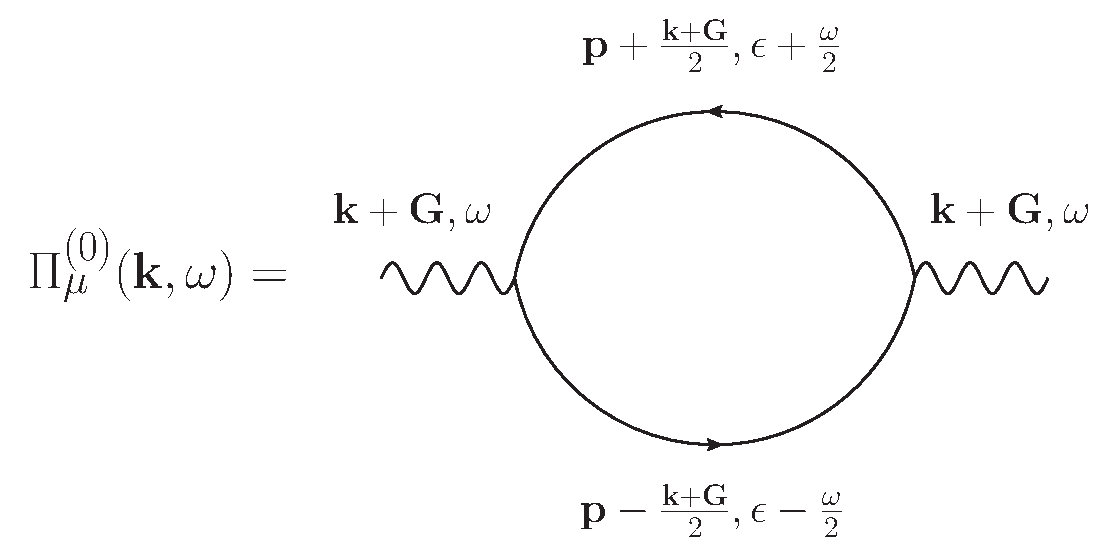
\includegraphics[width=0.5\textwidth]{bubble_diagram.eps}
	\caption{
This figure shows the first bubble diagram of the electronic polarization bubble caused by spin fluctuations.
The momentum ($\vb{k}+\vb{G}$) and frequency ($\omega$) transfer, originated from spin fluctuations, is divided on both fermionic lines (continous line).
	}
	\label{fig:bubble diagram}
\end{figure}
%
The bubble diagram is the lowest order of the full polarization operator.
In the following this diagram is computed in detail.
The first order of the polarization bubble is given by
%
\begin{align}
	\Pi_{\mu}^{(0)}(\vb{k}, \omega) = 
		i 
		\sum\limits_{\vb{P}}
		\int\limits_{|p| \leq |p_{\mt{F}}} \frac{\dd[2]{\vb{p}}}{(2\pi)^{2}} 
		\int\limits_{-\infty}^{\infty} \frac{\dd{\epsilon}}{2\pi}\,
		\mathcal{G}_{\mt{a}}^{(0)}(\vb{p}+\frac{\vb{k}}{2}, \epsilon+\frac{\omega}{2})
		\mathcal{G}_{\mt{b}}^{(0)}(\vb{p}-\frac{\vb{k}}{2}, \epsilon-\frac{\omega}{2}).
\end{align}
%
Here the outer momentum and frequency is shfited to symmetrizie the argument of both fermionic Green functions.
The Green function is given by
%
\begin{align}
	 \mathcal{G}_{\alpha}^{(0)}(\vb{k},\omega) := \green{\Psi_{\alpha}}{\Psi_{\alpha}^{\dag}}_{\omega} = \sum\limits_{\vb{G}} \frac{1}{\omega - \epsilon_{\alpha}(\vb{k}+\vb{G})}, 
	 \label{appeq:free electron propagator}
\end{align}
%
where the species of the corresponding fermions is indicated with the index $\alpha = \mt{a},\mt{b}$.
First of all, the dispersion relation of the fermions is investigated.
Spin fluctuations interact only with fermions near the Fermi surface.
Under this condition, the dispersion relation of the fermions of species a is expanded.
%
\begin{align}
	\epsilon_{\mt{a}}(\vb{p} + \frac{\vb{k} + \vb{G}}{2}) &= 
		\frac{\big(p_{x} + \frac{k_{x} + G_{x}}{2}\big)^{2}}{2m_{1}} 
		+ 
		\frac{\big(p_{y} + \frac{k_{y} + G_{y}}{2}\big)^{2}}{2m_{2}} 
		\notag \\ 
	\Leftrightarrow\ \epsilon_{\mt{a}}(\vb{p} + \frac{\vb{k} + \vb{G}}{2}) &=
		\frac{p_{x}^{2}}{2m_{1}} + \frac{1}{2} \frac{p_{x}}{m_{1}}(k_{x}+G_{x}) + \frac{(k_{x}+G_{x})^{2}}{8m_{1}}
		\notag \\ &+
		\frac{p_{y}^{2}}{2m_{2}} + \frac{1}{2} \frac{p_{y}}{m_{2}}(k_{y}+G_{y}) + \frac{(k_{y}+G_{y})^{2}}{8m_{2}}
		\notag \\
	\Leftrightarrow\ \epsilon_{\mt{a}}(\vb{p} + \frac{\vb{k} + \vb{G}}{2}) &\approx
		\xi_{\mt{a}} + \frac{1}{2} \vb{v}_{\mt{a,F}}(\vb{k} + \vb{G}) + \mu
\end{align} 
%
where the quadratic term with respect to $\vb{k}$ is neglected and $\xi_{\mt{a}}$ is the dispersion denoted in equation \eqref{eq:dispersion relations}.
Moreover, the velocity $\vb{v}_{a}$ of the fermion of species a is introduced.
Since only fermions near the Fermi surface are considered the velocity is assumed to be the Fermi velocity.
The same procudure is valid for the fermions of species b.
Finally, the normalized momentum vector $\vb{n} = \frac{\vb{p}}{|\vb{p}|}$ is introduced.
The Fermi velocity of fermions of species a is then given by $\vb{v}_{\mt{a,F}} = v_{\mt{a,F}} \vb{n}$ and equally for b.
The scalar product between the normalized momentum vector $\vb{n}$ and the bosonic spin density wave vector $\vb{k} + \vb{G}$ is rewriten as the magnitude multiplied with $\cos(\vartheta)$, where $\vartheta$ is the angle between both.

In the investigated model, the points of interaction between the fermions caused by spin fluctuations are hot-spots (see chapter \ref{ch:spin fermion model}).
This are certain points on the Fermi surface seperated by the momentum vector $\vb{Q}$.
The energy and the magnitudes of the Fermi velocities are equal on these points connected wby $\vb{Q}$.
%
\begin{align}
	\xi := \xi_{\mt{a}} = \xi_{\mt{b}} \qquad v_{\mt{F}} := v_{\mt{a,F}} = v_{\mt{b,F}}
\end{align}
%
The direction of the velocities have to be unequal
Otherwise, the angle $\vartheta$ is $0$ or $\pi$ and the imaginary part of $\Pi_{\mu}$ is zero.
Using these conversions and assumptions, the polarization operator is given by
%
\begin{align}
	\Pi_{\mu}^{(0)}(\vb{k}, \omega) &= 
		i \nu_{\mt{F}}
		\int\limits_{0}^{\pi} \dd{\vartheta}
		\int\limits_{\xi \leq \xi_{\mt{F}}} \dd{\xi}
		\int\limits_{-\infty}^{\infty} \frac{\dd{\epsilon}}{2\pi}
		\notag \\ &\times
		\frac{1}{\epsilon + \frac{\omega}{2} - \xi - \frac{1}{2} v_{\mt{F}} |\vb{k} + \vb{G}| \cos(\vartheta) + i \eta \sign(\epsilon + \frac{\omega}{2})}
		\notag \\ &\times
		\frac{1}{\epsilon - \frac{\omega}{2} - \xi + \frac{1}{2} v_{\mt{F}} |\vb{k} + \vb{G}| \cos(\vartheta) + i \eta \sign(\epsilon - \frac{\omega}{2})}.
	\label{appeq:pol operator before epsilon integration}
\end{align}
%
Here, the two dimensional momentum integral is firstly transformed in plane polar coordinates and then the $k$-integral is transformed into an energy integral over the density of states.
The density of states is approximated with the value of the density of states at the Fermi surface, $\nu_{\mt{F}} := \nu(\xi_{\mt{F}})$, since only fermions near the Fermi surface are considered.
The energy integral is limited by the Fermi energy $\xi_{\mt{F}}$.

The further treatment is started by computing the frequency integral.
The integral over $\epsilon$ is transformed into a complex contour integral, where the contour $\Gamma$ is chosen in two different ways.
According to the singularities of the integrand the countour is closed in the upper or lower half plane using a semicircle with radius infinity.
In both cases the contribution of the semicircle is zero, since the integrand is proportional to $\flatfrac{1}{\epsilon}$.
The equality between the integral along the real axis and the complex contour integral is ensured due to the non-contributing of the semicircle.
The investigated integrand has two singularities at
%
\begin{align}
	\epsilon_{1} := \xi - \frac{1}{2}\big(\omega - v_{\mt{F}} |\vb{k} + \vb{G}| \cos(\vartheta)\big) 
	\qq{and}
	\epsilon_{2} := \xi + \frac{1}{2}\big(\omega - v_{\mt{F}} |\vb{k} + \vb{G}| \cos(\vartheta)\big),
\end{align}
%
where both singularities are of first order.
The poles are located in the upper or lower plane, according to the signum function in the denominator.
In total four different constitutions are possible.
On the one hand, both singularities can be located in the lower or upper complex plane, which yield in both cases zero.
On the other hand, one pole is sited in the upper plane, while the other one is sited in the lower plane, or vice versa, where both yield the same contribution
%
\paragraph{1. case:} $\sign(\epsilon + \frac{\omega}{2}) = \sign(\epsilon - \frac{\omega}{2})$\\
%
Both singularities are located in the upper or in the lower complex half plane.
The contour is therefore closed in the upper or lower plane, respectivily, enclosing both poles .
In the first case the winding number is $1$, since the pole is enclosed counterclockwise.
Accordingly, the winding number is $-1$ in the second case.
%
\begin{align}
	&\mt{I}_{\omega}^{\mt{e}} := i \oint_{\Gamma} \frac{\dd{\omega}}{2\pi i}\, \frac{1}{\omega - \omega_{1} \mp i\eta} \cdot \frac{1}{\omega - \omega_{2} \mp i\eta}
	\notag \\
	\Leftrightarrow\ &\mt{I}_{\omega}^{\mt{e}} = \pm i \bigg[ \frac{1}{\omega_{2} - \omega_{1}} + \frac{1}{\omega_{1} - \omega_{2}}\bigg] = 0,
\end{align}
%
where the index "e" stands for even and means, that both poles are located in the same half plane.
%
\paragraph{2. case:} $\sign(\epsilon + \frac{\omega}{2}) \neq \sign(\epsilon - \frac{\omega}{2})$\\
%
The singularities are sited in different complex half planes, one in the upper and accordingly the other in the lower half plane.
It is arbitrary in which half plane the contour is closed as long as one pole is enclosed.
In the following computation the contour is closed in the upper half plane.
%
\begin{align}
	&\mt{I}_{\omega}^{\mt{o}} := i \oint_{\Gamma} \frac{\dd{\omega}}{2\pi i}\, \frac{1}{\omega - \omega_{1} \mp i\eta} \cdot \frac{1}{\omega - \omega_{2} \pm i\eta}
	\notag \\
	\Leftrightarrow\ &\mt{I}_{\omega}^{\mt{o}} = \frac{\pm i}{\omega_{2} - \omega_{1} \pm i\eta}
\end{align}
%
where the index "o" stands for odd and mean, that both poles are located in opposite half planes.

After inserting both expressions for the singularities $\omega_{1}$ and $\omega_{2}$, the intergand is independent with respect to $\xi$
The signum functions in \eqref{appeq:pol operator before epsilon integration} is equivalent to the signum functions $\sign(\xi \pm \frac{1}{2} v_{\mt{F}} |\vb{k} + \vb{G}| \cos(\vartheta))$ in energy representation.
The energy $\xi$ is dropped, since the integrand is independent of $\xi$, and the constant positive factors are neglectable. 
Then, the signum function is expressed as $\sign[|\vb{k} + \vb{G}| \cos(\vartheta))$.
Finally, the integrals limits are set to $\pm \frac{1}{2} v_{\mt{F}} |\vb{k} + \vb{G}| \cos(\vartheta)$, which follows directly from the localization of both poles.
$\omega_{1}$ is assumed to be in the lower half plane, while $\omega_{2}$ is then assumed in the opposite one.
This implies that $\epsilon + \frac{\omega}{2} > 0$ and $\epsilon - \frac{\omega}{2} < 0$, respectivily.
Transforming into energy representation the obtained expression yield the definition interval of $\xi$.
The polarization operator is therefore given by
%
\begin{align}
	\Pi_{\mu}^{(0)}(\vb{k}, \omega) &= 
		i \nu_{\mt{F}}
		\int\limits_{0}^{\pi} \dd{\vartheta} 
		\int\limits_{-\xi_{0}}^{\xi_{0}} \dd{\xi}
		\frac{i \sign(|\vb{k} + \vb{G}| \cos(\vartheta))}{\omega - v_{\mt{F}} |\vb{k} + \vb{G}| \cos(\vartheta) + i\eta \sign(|\vb{k} + \vb{G}| \cos(\vartheta))},
\end{align}
%
where the abbreviation $\xi_{0} = \flatfrac{v_{\mt{F}}|\vb{k}+\vb{G}|\cos(\vartheta)}{2}$ is introduced.
The integration over $\xi$ yields the factor $v_{\mt{F}}|\vb{k}+\vb{G}|\cos(\vartheta)$.
Subsequently the signum function is reexpressed in frequency representation corresponding to $\sign(\omega)$.
Since our interest is attracted to damping of the spin fluctuations, the imaginary part of the polarization operator is taken:
%
\begin{align}
	\Im{\Pi_{\mu}^{(0)}(\vb{k}, \omega)} &= 
		\nu_{\mt{F}} \pi
		\int\limits_{0}^{\pi} \dd{\vartheta}
		v_{\mt{F}} |\vb{k}+\vb{G}| \cos(\vartheta) \delta(\omega - v_{\mt{F}} |\vb{k} + \vb{G}| \cos(\vartheta)).
	\label{appeq:imaginary part of pol operator before theta integration}
\end{align}
%
Here the formula $\frac{1}{x \pm i\eta} = \PV{\frac{1}{x}} \mp i \pi \delta(x)$ is used.
The obtained $\delta$-distribution has a function $g(\vartheta)$  as argument.
Using formula
%
\begin{align}
	\delta(g(x)) = \sum\limits_{i=1} \frac{\delta(x-x_{0,i})}{|g'(x_{0,i})|},
\end{align}
%
the $\delta$-distribution is rewriten as a sum over $\delta$-distributions with the zeros of $g(\theta)$ as argument.
In the above formula, the sum runs over all zeros of $g(x)$, which are denoted as $x_{0,i}$.
The derivative with respect to $x$ is labeled with a prime at $g$ and is evaluated at the corresponding zero $x_{0,i}$.

In our observed case, the argument of $\delta(g(\vartheta))$ contains only one zero at \linebreak $\vartheta_{0} = \cos[-1](\flatfrac{\omega}{(v_{\mt{F}} |\vb{k} + \vb{G}|)})$ inside the integral boundaries.
The $\delta$-distribution is rewriten as:
%
\begin{align}
	&\delta(\omega - v_{\mt{F}} |\vb{k} + \vb{G}| \cos(\vartheta)) = \Big(v_{\mt{F}} |\vb{k} + \vb{G}| \cdot |\sin(\vartheta_{0})|\Big)^{-1} \delta(\vartheta - \vartheta_{0})
	\notag \\
	\Rightarrow\ &\delta(\omega - v_{\mt{F}} |\vb{k} + \vb{G}| \cos(\vartheta)) \approx \Big(v_{\mt{F}} |\vb{k} + \vb{G}|\Big)^{-1} \delta(\vartheta - \vartheta_{0}).
\end{align}
%
In the second line the limit of small frequancies $\omega$ is taken, which is valid in our observed low-energy theory in the spin fermion model.
The integration over $\vartheta$ is now performed and the imaginary part of the polarization operator is given by
%
\begin{align}
	\Im{\Pi_{\mu}^{(0)}(\vb{k}, \omega)} &= \frac{\nu_{\mt{F}} \pi}{v_{\mt{F}} |\vb{k} + \vb{G}|} \cdot \omega = \gamma \omega,	 
\end{align}
%
where the damping parameter $\gamma$ is introduced.
As above demonstrated, the damped spin density propagator is determined by the Dyson equation \eqref{appeq:Dyson equation}.
The polarization operator is reperated into real and imaginary part.
Inserting the free spin density propagator and the obtained result for $\Im{\Pi_{\mu}}$, the damped spin density popagator is obtained to
%
\begin{align}
	\mathcal{D}_{\mu}(\vb{k}, \omega) = \sum\limits_{\vb{G}} \frac{1}{(\vb{k}+\vb{G})^{2} + r - (\flatfrac{\omega}{v_{\mt{S}}})^{-2} - i \gamma \omega}
	\label{appeq:damped spin density propagator with real omega}
\end{align}
%
where the abbreviation $r = r_{0} - \Re{\Pi_{\mu}(\vb{k}, \omega)}$ is used.
In the vicinity of the quantum critical point the real part of $\Pi_{\mu}$ is canceled by $r_{0}$, since the correlations length is divergent and $r=\xi^{-2}$
In low-energy theory, the $\omega^{2}$-term is further neglectable.
%
%
\section{Transformation into Matsubara Frequency Space}
\label{appsec:transformation into Matsubara frequency space}
%
%
The spin density wave propagator, obtained in the previous section, is a complex function of the real quantity $\omega$.
In the following, the quantity $\omega$ is transformed into an imaginary quantity $i\omega_{n}$, known as Matsubara frequancies.
The real and imaginary part of the propagator $\mathcal{D}_{\mu}(\vb{k}, i\omega_{n})$ with respect to Matsubara frequencies is evaluated using the Kramers-Kronig relations \cite{Schwabl}.
The propagator in \eqref{appeq:damped spin density propagator with real omega} is seperated into real and imaginary part, extending with the complex conjugated denominater.
%
\begin{align}
	\mathcal{D}_{\mu}(\vb{k}, \omega) = \sum\limits_{\vb{G}} \bigg[\frac{(\vb{k}+\vb{G})^{2}}{(\vb{k}+\vb{G})^{4} + (\gamma\omega)^{2}} + i \frac{\gamma \omega}{(\vb{k}+\vb{G})^{4} + (\gamma\omega)^{2}}\bigg],
	\label{appeq:real and imaginary part of D}
\end{align}
%
where $r$ and $\xi$ is set to zero.
For the following treatment it is usefull to investigate the symmetries of the real and imaginary part.
The real part is a symmetric function and the imaginary part is an antiysmmetric funtion, with respect to $\omega$.
The imarginary part of $\mathcal{D}_{\mu}(\vb{k}, i\omega_{n})$ is evaluated to zero, since its defined as the integral over the real part of $\mathcal{D}_{\mu}(\vb{k}, \omega)$ divided by $\omega$.
The integrand is therefore an odd function and the integral over all frequencies $\omega$ is zero.
In Matsubara frequency space, the damped propagator is given by its real part.
%
\begin{align}
	\mathcal{D}_{\mu}(\vb{k}, i\omega_{n}) = \Re{\mathcal{D}_{\mu}(\vb{k}, i\omega_{n})} = \frac{1}{\pi}\: \PV{\int\limits_{-\infty}^{\infty} \dd{\omega} \frac{\Im{\mathcal{D}_{\mu}(\vb{k}, \omega)}}{\omega - i\omega_{n}}}
\end{align}
%
where $\PV$ represents that the integrals is evaluated using the principal value.
The integral is speperated into two parts. 
In the first one $\omega$ is substituted by $-\omega$ and the antismmetry of $\Im{\mathcal{D}_{\mu}(\vb{k}, \omega)}$ is utilizied.
%
\begin{align}
	&\mathcal{D}_{\mu}(\vb{k}, i\omega_{n}) = \frac{1}{\pi} \int\limits_{0}^{\infty} \dd{\omega} \Im{\mathcal{D}_{\mu}(\vb{k}, \omega)} \Bigg[
		\frac{1}{\omega + i\omega_{n}}
		+
		\frac{1}{\omega - i\omega_{n}}
	\Bigg]
	\notag \\
	\Leftrightarrow\ &\mathcal{D}_{\mu}(\vb{k}, i\omega_{n}) = 
		\frac{2}{\pi} \sum\limits_{\vb{G}} \int\limits_{0}^{\infty} \dd{\omega} 
		\frac{\gamma \omega}{(\vb{k}+\vb{G})^{4} + (\gamma\omega)^{2}} \cdot
		\frac{\omega}{\omega^{2} + \omega_{n}^{2}}
	\notag \\
	\Leftrightarrow\ &\mathcal{D}_{\mu}(\vb{k}, i\omega_{n}) = 
		\sum\limits_{\vb{G}} \frac{1}{(\vb{k}+\vb{G})^{2} + \gamma|\omega_{n}|}
	\label{eq: damped propagator Matsubara representation}
\end{align}
%
In the last step the integral formula
%
\begin{align}
	\int\limits_{0}^{\infty} \dd{x} \frac{x}{a^{2} + x^{2}} \cdot \frac{x}{y^{2} + x^{2}} = \frac{\pi}{2} \frac{1}{a + |y|}
\end{align}
%
is used, which can be shown by transforming into a complex contour integral.

















%The spin fermion model considers an interaction between electrons on different Fermi surfaces, where the interaction is originated by spin density waves.
%On that reason the propagation of the spin density waves is damped.
%The damping should be considered in the propagator via doing pertubation theory.

%Because the damping is originated by the interaction between electrons the free electron propagator is also needed in the following calculation.
%The propagator can be calculated in the same way as the  one for free spin density waves.
%This handwork shouldn't be done here explicitly.
%The free electron propagator is given by
%
%\begin{align}
%	 \mathcal{G}_{\alpha}^{(0)}(\vb{k},\omega) := \green{\Psi_{\alpha}}{\Psi_{\alpha}^{\dag}}_{\omega} = \sum\limits_{\vb{G}} \frac{1}{\omega - \epsilon_{\alpha}(\vb{k}+\vb{G})}, 
%	 \label{eq: free electron propagator}
%\end{align}
%
%where $\alpha = \mt{a,b}$ denotes the Fermi surface of the respective electrons.
%The damped spin density wave propagator is computed using the usually method of pertubation theory in quantum field theory.



